%%
%% Copyright 2007, 2008, 2009 Elsevier Ltd
%%
%% This file is part of the 'Elsarticle Bundle'.
%% ---------------------------------------------
%%
%% It may be distributed under the conditions of the LaTeX Project Public
%% License, either version 1.2 of this license or (at your option) any
%% later version.  The latest version of this license is in
%%    http://www.latex-project.org/lppl.txt
%% and version 1.2 or later is part of all distributions of LaTeX
%% version 1999/12/01 or later.
%%
%% The list of all files belonging to the 'Elsarticle Bundle' is
%% given in the file `manifest.txt'.
%%
%% Template article for Elsevier's document class `elsarticle'
%% with harvard style bibliographic references
%% SP 2008/03/01
%%
%%
%%
%% $Id: elsarticle-template-harv.tex 4 2009-10-24 08:22:58Z rishi $
%%
%%
\documentclass[preprint,authoryear,12pt]{elsarticle}

%% Use the option review to obtain double line spacing
%% \documentclass[authoryear,preprint,review,12pt]{elsarticle}

%% Use the options 1p,twocolumn; 3p; 3p,twocolumn; 5p; or 5p,twocolumn
%% for a journal layout:
%% \documentclass[final,authoryear,1p,times]{elsarticle}
%% \documentclass[final,authoryear,1p,times,twocolumn]{elsarticle}
%% \documentclass[final,authoryear,3p,times]{elsarticle}
%% \documentclass[final,authoryear,3p,times,twocolumn]{elsarticle}
%% \documentclass[final,authoryear,5p,times]{elsarticle}
%% \documentclass[final,authoryear,5p,times,twocolumn]{elsarticle}

%% if you use PostScript figures in your article
%% use the graphics package for simple commands
%% \usepackage{graphics}
%% or use the graphicx package for more complicated commands
%% \usepackage{graphicx}
%% or use the epsfig package if you prefer to use the old commands
%% \usepackage{epsfig}

%% The amssymb package provides various useful mathematical symbols
\usepackage{graphicx}
\usepackage{epstopdf}
\usepackage{amssymb}
\usepackage{amsmath}
%\usepackage{a4wide}
\usepackage{color}
%\usepackage{subcaption}
\newcommand{\hilight}[1]{\colorbox{yellow}{#1}}
%% The amsthm package provides extended theorem environments
%% \usepackage{amsthm}
\newcommand\solidrule[1][1cm]{\rule[0.5ex]{#1}{1pt}}
\newcommand\dashedrule{\mbox{\solidrule[1mm]\hspace{1mm}\solidrule[1mm]\hspace{1mm}\solidrule[1mm]\hspace{1mm}}}

\newcommand{\ustar}{\ensuremath{U^{*}}}
\newcommand{\cstar}{\ensuremath{c^{*}}}
\newcommand{\reynoldsnumber}{\ensuremath{Re}}
\newcommand{\massstiff}{\ensuremath{\Pi_1}}
\newcommand{\massdamp}{\ensuremath{\Pi_2}}


\newcommand{\Tan}[1]{{\textcolor{blue}{{\bf{\it{ **Tan: #1 **}}}}}}
\newcommand{\JL}[1]{{\textcolor{red}{{\bf{\it{ **JL: #1 **}}}}}}

%% The lineno packages adds line numbers. Start line numbering with
%% \begin{linenumbers}, end it with \end{linenumbers}. Or switch it on
%% for the whole article with \linenumbers after \end{frontmatter}.
%% \usepackage{lineno}

%% natbib.sty is loaded by default. However, natbib options can be
%% provided with \biboptions{...} command. Following options are
%% valid:

%%   round  -  round parentheses are used (default)
%%   square -  square brackets are used   [option]
%%   curly  -  curly braces are used      {option}
%%   angle  -  angle brackets are used    <option>
%%   semicolon  -  multiple citations separated by semi-colon (default)
%%   colon  - same as semicolon, an earlier confusion
%%   comma  -  separated by comma
%%   authoryear - selects author-year citations (default)
%%   numbers-  selects numerical citations
%%   super  -  numerical citations as superscripts
%%   sort   -  sorts multiple citations according to order in ref. list
%%   sort&compress   -  like sort, but also compresses numerical citations
%%   compress - compresses without sorting
%%   longnamesfirst  -  makes first citation full author list
%%
%% \biboptions{longnamesfirst,comma}

% \biboptions{}

\journal{Journal of Fluid Structures}

\begin{document}
\begin{frontmatter}

%% Title, authors and addresses

%% use the tnoteref command within \title for footnotes;
%% use the tnotetext command for the associated footnote;
%% use the fnref command within \author or \address for footnotes;
%% use the fntext command for the associated footnote;
%% use the corref command within \author for corresponding author footnotes;
%% use the cortext command for the associated footnote;
%% use the ead command for the email address,
%% and the form \ead[url] for the home page:
%%
%% \title{Title\tnoteref{label1}}
%% \tnotetext[label1]{}
%% \author{Name\corref{cor1}\fnref{label2}}
%% \ead{email address}
%% \ead[url]{home page}
%% \fntext[label2]{}
%% \cortext[cor1]{}
%% \address{Address\fnref{label3}}
%% \fntext[label3]{}

\title{A study on the energy transfer of a square prism under fluid-elastic galloping}

%% use optional labels to link authors explicitly to addresses:
%% \author[label1,label2]{<author name>}
%% \address[label1]{<address>}
%% \address[label2]{<address>}

\author{H.G.K.G. Jayatunga, B.T. Tan, J. S. Leontini}

\address{}

\begin{abstract}
Extracting useful energy from flow induced vibrations has become a developing area of research in recent years. In this paper, we analyse power transfer of an elastically mounted body under the influence of fluid-elastic galloping. The system and the power transfer is analysed by numerically integrating the quasi-steady state model equations. The power transfer is analysed for both high ($\reynoldsnumber=22300$) and low ($\reynoldsnumber=200$) Reynolds numbers cases.

At high mass ratios ($m^*>50$), the power transfer is completely controlled by galloping and essentially independent of the mass. A combined mass-damping coefficient, \massdamp, that can be derived from the equation of motion, is shown to be the parameter that governs power output. The system is a balance between the power delivered to the system due to fluid-dynamic forcing and power removed through mechanical damping which are governed by the fluid-dynamic forcing characteristics (i.e. the lift force as a function of incident angle) and mechanical damping coefficient respectively. Comparing the DNS results with the QSS data  uncovered that a good agreement of the data could be obtained even at low Reynolds numbers when the inertia of the system (mass ratio) is substantially high.    



\end{abstract}

\begin{keyword}
%% keywords here, in the form: keyword \sep keyword

%% MSC codes here, in the form: \MSC code \sep code
%% or \MSC[2008] code \sep code (2000 is the default)

\end{keyword}

\end{frontmatter}

% \linenumbers

%% main text
\section{Introduction} 
 
Fluid-elastic galloping is one of the sub-areas of research in fluid structure interactions. This area has been of interest due to the vibrations crated by galloping on transmission lines and civil structures and leading them to failure. Therefore understanding this phenomenon in order to suppresses these vibrations was quite important. However, the search for alternate energy sources with minimal environmental impact has become an important area of research in the modern word. Therefore researchers are moving towards investigating the possibility of extracting useful energy from this vibrations rather than suppressing them. Thus, it is quite important to understand the governing parameters and analyse the influence of them on the energy transfer from the fluid to the structure, because this understanding will lead to develop better practical applications. Hence, in this paper we focus on understanding the energy transfer from the fluid to the body and isolate the governing parameters influencing it.

According to \citet{Paidoussis2010}, \citet{Glauert1919} provided a criterion for galloping by considering the auto-rotation of an aerofoil.  \citet{DenHartog1956} provided a theoretical explanation for galloping for iced electric transmission lines. A weakly non-linear theoretical aeroelastic model to predict the response of galloping was developed by \citet{Parkinson1964} based on the quasi-steady state hypothesis. Experimental lift and drag data on a fixed square prism at different angles of attack were used as an input for the theoretical model. It essentially used a curve fit of the transverse force to predict the galloping response. The study managed to achieve a good agreement with experimental data.

However, the QSS model equation when solved analytically using the sinusoidal solution, cannot predict the response for cases with low mass ratios. \citet{Joly2012} observed that finite element simulations show a sudden change in amplitude below a critical value of the mass ratio. The quasi-oscillator equation in \citet{Parkinson1964} was altered to account for the vortex shedding and solved numerically to predict the reduced displacement amplitude at low mass ratios to the point where galloping is no longer present. \citet{Barrero-Gil2010a} investigated the possibility of extracting power from vibrations caused by galloping using the quasi-steady state model. So far the studies on galloping using quasi-steady state assumption has been mainly focused on understanding the behaviour of the displacement amplitude. Although, it is quite important to analyse the behaviour of the velocity when studying the power transfer from the fluid to the body. This is because power could be simply defined as the product the force and velocity. This study also focuses on how well the QSS model perform at high damping at low Reynolds numbers. 


Here, the modified QSS model is integrated numerically for low Reynolds numbers. The power transfer from the fluid to the structure and the influence of mechanical parameters was investigated (i.e. mass, stiffness and damping). To this end, a series of previously mentioned mechanical parameters are tested at two different values of \reynoldsnumber: $\reynoldsnumber = 200$, a case that should remain laminar and closer to two-dimensional behaviour; $\reynoldsnumber = 22300$, a case where the flow is expected to be turbulent and three-dimensional. Both cases require the input of transverse force coefficients $C_y$ as a function of angle of attack $\theta$ for a fixed body. These data are provided from direct numerical simulations for the $\reynoldsnumber = 200$ case, while the data provided by \citet{Parkinson1964} are used for the $\reynoldsnumber = 22300$ case.

The structure of the paper is as follows. Section \ref{sec:theory} presents the governing equations and the oscillator model used to obtain data and introduces the method for the calculation of the power transferred from the fluid to the structure. Section \ref{sec:results} introduces the governing parameters namely, the combined mass-stiffness and the combined mass-damping obtained using linearised time scales of the oscillator model. The fixed body tests at a range of $\theta$ followed by the response characteristics predicted by the integration of the QSS model for both the high and low \reynoldsnumber\ cases. For the low \reynoldsnumber\ case, the results of the QSS model are compared to those of full direct numerical simulations of the fluid-structure interaction problem. Finally, section \ref{sec:conc} presents the conclusions that can be drawn from this work.
% % % % % % % % % % % % % % % % % % % % % % % % % % % % % % % % % % % % % % % % % % % % % % % % % % % % % % % % % % % % % % % % % % % % % % % % 
\section*{Nomenclature}
%\textbf{Nomenclature}

\begin{tabular}{ll}
$a_1,a_3,a_5,a_7$ & coefficients of the polynomial to determine $C_y$ \\ 
$A$ & displacement amplitude\\
$c$ & damping constant \\
$D$ & characteristic length (side length) of the cross section of the body \\
$f=\sqrt{k/m}/2\pi$ & natural frequency of the system \\
$F_y$ & instantaneous force normal to the flow \\ 
$F_0$& amplitude of the oscillatory force due to vortex shedding \\
$k$ & spring constant \\
$m$ & mass of the body \\
$m_a$ & added mass \\
$P_d$ & power dissipated due to mechanical damping  \\
$P_{in}=\rho U^3D/2$ & Energy flux of the approaching flow \\
$P_{mean}$ & mean power \\
$P_t$   & power transferred to the body by the fluid \\
$t$ & time \\
$U$ & freestream velocity \\
$U_i$ & Induced velocity \\
$y,\dot{y},\ddot{y}$ & transverse displacement, velocity and acceleration of the body \\
$\mathcal{A}=DL$ & frontal area of the body\\ 
$\lambda$ & Inverse time scale of a galloping dominated flow \\
$\lambda_{1,2}$ & Eigenvalues of linearized equation of motion \\
$\rho$ & fluid density  \\
$\omega_n= 2 \pi f$ & natural angular frequency of the system  \\
$\omega_s$ & vortex shedding angular frequency \\
$\cstar=cD/mU$ & non-dimensionalised damping factor \\
$C_y=F_y/0.5\rho U^2DL$ & normal (lift) force coefficient \\
$m^*=m/\rho D^2L$ & mass ratio \\
$Re$ & Reynolds number  \\
$U^*=U/fD$ & reduced velocity  \\
$Y=y/D$ & non-dimensional transverse displacement \\
$\dot{Y}=m^*\dot{y}/a_1U$ & non-dimensional transverse velocity \\
$\ddot{Y}=m^{*2}D/a_1^2U^2$ & non-dimensional transverse acceleration \\
$\Gamma_1 = 4\pi^2m^{*2}/U^{*2}a_1^2$ & First dimensionless group arising from linearised, non-dimensionalised equation of motion\\
$\Gamma_2 = c^*m^*/a_1$ & Second dimensionless group arising from linearised, non-dimensionalised equation of motion\\
$\zeta= c/2 m \omega_n$ & damping ratio \\
$\theta= \tan^{-1}{(\dot{y}/U)}$ & instantaneous angle of incidence (angle of attack)\\
$\massstiff =  4\pi^2m^{*2}/U^{*2}$ & Combined mass-stiffness parameter\\
$\massdamp = c^*m^*$ & Combined mass-damping parameter\\
\end{tabular}  


% % % % % % % % % % % % % % % % % % % % % % % % % % % % % % % % % % % % % % % % % % % % % % % % % % % % % % % % % % % % % % % % % % % % % % % % % % % %

\section{Problem formulation and methodology}
\label{sec:theory}

\subsection{The quasi-steady state (QSS) model}

The equation of motion of the body is given by 
\begin{equation}
\label{equationofmotion}
(m)\ddot{y}+c\dot{y}+ky=F_y,
\end{equation}
where the forcing term $F_y$ is given by
\begin{equation}
\label{lift equation}
F_y=\frac{1}{2}\rho U^2\mathcal{A}C_y.
\end{equation}


\begin{figure}
\setlength{\unitlength}{\textwidth}

  \begin{picture}(1,0.23)(0,0.74)
    
  \put(0.2,0.76){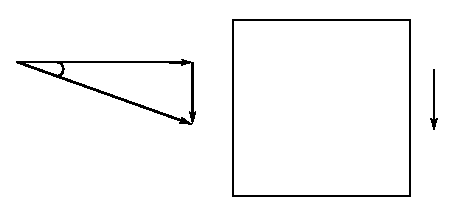
\includegraphics[width=0.5\unitlength]{../FnP/gnuplot/setup-1.eps}}         
      
      
   
 	\put(0.315,0.93){$U$}
 	\put(0.3,0.84){$U_i$}
    \put(0.42,0.88){$\dot{y}$}
    \put(0.28,0.895){ $\theta$}
    \put(0.7,0.87){\small $(+)$}
      	

 	
 	 

     

  \end{picture}

 \caption{Induced angle of attack on the square prism due to the resultant of free-stream velocity of the fluid and transverse velocity of the body.}
    \label{fig:setup_1}
\end{figure}

In the QSS model, it is assumed that the force on the body at a given instantaneous incident angle $\theta$ (defined in figure \ref{fig:setup_1}) is the same as the mean force on a static body at the same incident angle, or angle of attack. The instantaneous value of $C_y$ is therefore determined by an interpolating polynomial based on the lift data for flow over a stationary body at various $\theta$. Using the relationship between $\theta$ and the instantaneous transverse velocity of the body $\dot{y}$ shown in figure \ref{fig:setup_1}, $C_y$ can be written as a function of $\dot{y}$. The order of the interpolation polynomial used to define this function has varied from study to study. For  example a $7^{th}$ order polynomial was used in \cite{Parkinson1964} and $3^{rd}$ order polynomial was used in \cite{Barrero-Gil2009}. \cite{Ng2005} concluded that using a $7^{th}$ order polynomial is sufficient and a polynomial higher than that of $7^{th}$ order doesn't provides a significantly better result. Thus a $7 ^{th}$ order interpolating polynomial is used in this present study. As a result, $C_y(\theta)$ (noting that theta is proportional to $\dot{y}/U$) is defined as
\begin{equation}
\label{cy ploynomial}
C_y(\theta)=a_1\left(\frac{\dot{y}}{U}\right)+a_3\left(\frac{\dot{y}}{U}\right)^3+a_5\left(\frac{\dot{y}}{U}\right)^5+a_7\left(\frac{\dot{y}}{U}\right)^7.
\end{equation}

%\begin{equation}
%\label{modified_equation_of_motion}
%\ddot{y}+c^*\dot{y}+k^*y=\frac{1}{2}\rho U^2A
%\end{equation}

 It is expected that vortex shedding will be well correlated along the span and provide significant forcing at low \reynoldsnumber. \citet{Joly2012} introduced  an additional sinusoidal forcing function to the hydrodynamic forcing to model this. This enables the model to provide accurate predictions even at low mass ratios where galloping excitation is suppressed or not present. However, in this study we also focus on isolating the regions where the QSS model predicts well and therefore the additional sinusoidal forcing function is disregarded.  
 
 
 
\begin{equation}
\label{final_equation_motion}
m\ddot{y}{+}c\dot{y}{+}ky{=}\frac{1}{2}\rho U^2 \mathcal {A} \Bigg(a_1\left(\frac{\dot{y}}{U}\right){+}a_3\left(\frac{\dot{y}}{U}\right)^3{+}a_5\left(\frac{\dot{y}}{U}\right)^5{+}a_7\left(\frac{\dot{y}}{U}\right)^7.
\end{equation}

This equation can be solved using standard time integration methods. In this study the fourth-order Runge-Kutta scheme built in to the MATLAB routine `ode45' was generally used to obtain the solutions. 

\subsection{Calculation of average power}

 The dissipated power due to the mechanical damping represents the ideal potential amount of harvested power output. Therefore, the mean power output can be given by
\begin{equation}
\label{power}
P_{mean}=\frac{1}{T}\int_{0}^{T}(c\dot{y})\dot{y} dt,
\end{equation}
where $T$ is the period of integration and $c$ is the mechanical damping constant. 

It should be noted that this quantity is equal to the work done on the body by the fluid, defined as
\begin{equation}
\label{power_alt}
P_{mean}=\frac{1}{T}\int_{0}^{T}F_y\dot{y} dt,
\end{equation}
where $F_y$ is the transverse (lift) force.

 \hilight{have to repharase} These two definitions show two important interpretations of the power with respect to any energy production device. The first shows that power will be high for situations where the damping coefficient is high, and the transverse velocity is consistently high. The second shows that power will be high for situations where the transverse force and the body velocity are in phase.
 
 \begin{figure}

  \setlength{\unitlength}{\textwidth}
  \begin{picture}(1,0.25)(0,0.8)
  
    % % %90
      \put(0.025,0.81){\includegraphics[width=0.5\unitlength]{./chapter-pi_1_pi_2/FnP/gnuplot/lift_curve_200.eps}}
      \put(0.495,0.81){\includegraphics[width=0.5\unitlength]{./chapter-pi_1_pi_2/FnP/gnuplot/lift_curve_park.eps}}
 	\put(0.02,0.93){ \large $C_y$} 	
% 	\put(0.56,1.02){ $\theta$}
 	
        \put(0.25,0.8){ $\theta$} 	
        \put(0.75,0.8){ $\theta$}
        
        \put(0.117,1.01){(a)}
        \put(0.565,1.01){(b)}
      \end{picture}

  \caption{Lift coefficient, $C_y$, as a function of incidence angle $\theta$, for a static square cross section. (a) Data from simulations at $Re=200$  (b) data from \cite{Parkinson1964} at $Re=22300$. Points ($\bullet$) are measurements from the simulations. At $\reynoldsnumber=200$. Curves in both plots are 7th-order interpolating polynomials used to predict the fluid forcing for the QSS model. $C_y$ is the force coefficient of the force which occurs normal to the induced velocity.}
    \label{fig:lift_curves}
\end{figure}


 \begin{table}[ht]

\begin{center}
\setlength{\unitlength}{\textwidth}

\begin{tabular}{c c c c c} % centered columns (4 columns)
\hline\hline %inserts double horizontal lines
\\[0.2ex]
Case & $a_1$ & $a_3$ & $a_5$ & $a_7$ \\ [0.8ex] % inserts table 
%heading
\hline 
\\[0.8ex]% inserts single horizontal line
Re=200 & 2.32 & 197.8 & 4301.7 & 30311.9 \\[0.8ex]% inserting body of the table
Re=22300 & 2.69 & 168 & 1670 & 59900 \\ [1ex] % [1ex] adds vertical space
\hline %inserts single line
\end{tabular}

\caption{Coefficient values used in the 7th order interpolation polynomial for high ($Re=22300$) and low ($Re=200$) Reynolds numbers. These data are used as input data to calculate the right-hand side of Eq. \ref{final_equation_motion} throughout this study.}
 
\label{table:cy-coefficients} % is used to refer this table in the text
\end{center}
\end{table}


 
 \subsection{Parameters used} 
  
 For the low \reynoldsnumber\ tests, $\reynoldsnumber=200$ was maintained. Stationary $C_y$ data were obtained at different angles of attack ranging from $0^\circ$ to $16^\circ$. The average power was obtained by using equation \ref{power}, and the averaging was done over no less than 20 galloping periods. Predictions of power output at $\reynoldsnumber=22300$ were obtained using the coefficients for curve fitting $C_y$ (Table (\ref{table:cy-coefficients})) from \citet{Parkinson1964}, in order to provide a comparison between high and low Reynolds numbers. The mass ratio $m^*$ was kept at 1163 for $\reynoldsnumber=22300$ (Similar to \citet{Parkinson1964}) and $m^*=20$ for \reynoldsnumber=200. These parameters were used throughout this study unless otherwise specified. 
 
 The stationary data and the fluid-structure interaction (FSI) data were obtained using a high-order spectral element routine to simulate the two-dimensional laminar flow.  Simulations involving fluid structure interaction (FSI) were used to provide additional validation of the QSS model. The inlet was placed $20D$ while the outlet situated $60D$ away from the centroid of the body. The side boundaries were placed $20D$ away from the centroid of the body where $D$ was kept as unity throughout this study. The Navier--Stokes equations were solved in an accelerated frame of reference attached to the moving body along with the body equation of motion given in equation \ref{equationofmotion}. A three-step time splitting scheme together with high-order Lagrangian polynomials were used to obtain the solution. The details of the method can be found in \citet{Thompson2006,Thompson1996a}. This code has been very well validated in a variety of fluid-structure interaction problems \citep{Leontini2007a,Griffith2011,Leontini2011,Leontini2013}.
  
 The computational domain consists of 751 quadrilateral macro elements where the majority of the elements were concentrated near the square section. A freestream condition was given to the inlet, top and bottom boundaries and the normal velocity gradient was set to zero at the outlet. A convergence study was performed by changing the order of the polynomial ($p$-refinement) at $U^*=40$ and $\reynoldsnumber=200$. A $9^{th}$ order polynomial together with a time step of $\Delta tU/D=0.001$ was sufficient to ensure an accuracy of $2\%$ with regards to amplitude of oscillation.
 
 
 
 % % % % % % % % % % % % % Time scales % % % % % % % % % % % % % % % % % % % % % % % % % % % % % % %
 
 \section{Results}
  \label{sec:results}
  
     Figure \ref{fig:lift_curves} shows the plots of the interpolation polynomials as a function of $\theta$. For high \reynoldsnumber \ the polynomial incorporated by \cite{Parkinson1964} was used. For low \reynoldsnumber \ two polynomials were used to obtain a better fit to the data. One to fit data from $\theta=0^0 \rightarrow 7^0$ and the other $\theta > 7^0$ 
   there are several differences that can be observed when the low \reynoldsnumber\ data are compared with the $7^{th}$ order polynomial curve at $\reynoldsnumber=22300$ shown in figure \ref{cy ploynomial}(b). The peak value of $C_y$ is  significantly lower at $\reynoldsnumber=200$ ($C_y=0.12$ at $5^\circ$) in comparison with $\reynoldsnumber=22300$ ($C_y=0.57$ at $13^\circ$) . The inflection point present around $8^\circ$ for $\reynoldsnumber=22300$ is not observed at $\reynoldsnumber=200$. This agrees with the findings of \cite{Luo2003}.  It was concluded by \cite{Luo2003} that hysteresis in the system response occurs due to the inflection point in the $C_y$ curve. Therefore hysteresis is not expected at $\reynoldsnumber=200$.
  
   
  The range of incident flow angles where $C_y$ remains positive is narrow at $\reynoldsnumber=200$ ($0^\circ <\theta \leq$ $7^\circ$) compared to $\reynoldsnumber=22300$ ($0^\circ <\theta \leq 15^\circ$). This feature is what sustains galloping. Power is only transferred from the fluid to the supporting structure within this range of incident angles because fluid forces are acting in the direction of travel of the oscillating body, as demonstrated by equation \ref{power_alt}. Incident angles beyond this range actually suppress the galloping and power goes in the opposite direction, i.e; from body to fluid. Therefore due to the overall smaller $C_y$ and narrow range of angles where $C_y$ is positive for $\reynoldsnumber=200$ compared to $\reynoldsnumber=22300$, it is expected that the transferred power at $\reynoldsnumber=200$ is significantly lower than at $\reynoldsnumber=22300$.
  
 
  \begin{figure}
  \setlength{\unitlength}{\textwidth}

  \begin{picture}(1,0.72)
%(0,0.35)
    
    % % %Parkinson Data 
    \put(0.025,0.48){\includegraphics[width=0.5\unitlength]{../FnP/gnuplot/displacement_amp_re_parkinson_1.eps}}
    \put(0.025,0.25){\includegraphics[width=0.5\unitlength]{../FnP/gnuplot/velocity_amp_re_parkinson.eps}}
    \put(0.025,0.02){\includegraphics[width=0.5\unitlength]{../FnP/gnuplot/mean_power_re_parkinson.eps}}
    
    % Re 165 Data 
    \put(0.495,0.48){\includegraphics[width=0.5\unitlength]{../FnP/gnuplot/displacement_amp_re200.eps}}
    \put(0.495,0.25){\includegraphics[width=0.5\unitlength]{../FnP/gnuplot/velocity_amp_re200.eps}}
    \put(0.495,0.02){\includegraphics[width=0.5\unitlength]{../FnP/gnuplot/mean_power_re_200.eps}}
   
%    \put(0.25,0.93){\ustar}
%    \put(0.8,0.93){\ustar}
%    \put(0.25,0.63){\ustar}
%   \put(0.8,0.63){\ustar}
    \put(0.25,0.0){\ustar}
    \put(0.75,0.0){\ustar}
    
    \put(0.00,0.6){$\displaystyle\frac{A}{D}$}
%    \put(0.52,1.075){$\frac{A}{D}$}
    \put(0.00,0.4){$\displaystyle\frac{V}{D}$}
%    \put(0.52,0.83){$\frac{V}{D}$}
    \put(-0.025,0.15){$\displaystyle\frac{P_{m}}{\rho \mathcal{A}U^3 }$}
%    \put(0.5,0.54){$\frac{P_{m}}{\rho \mathcal{A}U^3 }$}
    
    \put(0.085,0.685){\small(a)}
    \put(0.555,0.685){\small(b)}
    \put(0.085,0.455){\small(c)}
    \put(0.555,0.455){\small(d)}
    \put(0.085,0.225){\small(e)}
    \put(0.555,0.225){\small(f)}   
  \end{picture}

%  \vspace{-4cm}
  \caption{Velocity amplitude, displacement amplitude and mean power  as functions of $U^*$. Data presented in (a), (c) and (e) were calculated using input data at $Re=22300$ and $m^*=1163$ obtained by \cite{Parkinson1964} at three different damping ratios: $\zeta=0.0125$ (\ding{83}), $\zeta=0.015$ (\ding{116}) and $\zeta=0.0175$ (\ding{108}). Data presented in (b),(d) and (f) were obtained using input data at $Re=200$ and $m^*=20$ at three different damping ratios: $\zeta=0.075$ ($\times$), $\zeta=0.1$ (\ding{117}) and $\zeta=0.15$ (+). The multiple branches for the higher Re are due to the hysteresis between two solutions.}
  
\label{fig:uncollapsed_data}
\end{figure}



      
        
    The quasi-steady analysis data reveal that the displacement amplitude grows with increasing $U^*$. This is shown for both the high and low \reynoldsnumber\ cases in figures \ref{fig:uncollapsed_data} (a) and (b). The onset of galloping is delayed with increasing damping ratio $\zeta$ for both high and low Reynolds numbers. These results are consistent with the earlier studies by \cite{Parkinson1964} and \cite{Barrero-Gil2010a}. Hysteresis could be observed for the case with a higher Reynolds number. Different solutions could be obtained by manipulating the initial conditions (initial displacement) of the system. The upper branch was obtained by giving an initial displacement which was higher than the expected amplitude while the lower branch was obtained by providing a lower initial displacement than the expected amplitude. Although theory shows a possible third state, it is an unstable branch and as such it could not be achieved numerically. This was also observed by \cite{Vio2007}. It could be observed ( Figure \ref{fig:uncollapsed_data}) that the power peaks at different \ustar \ at different $\zeta$. However, unlike VIV, galloping is not dependent on frequency but on the induced velocity. Data presented in \citet{Barrero-Gil2010a} are presented in the classical VIV parameters (i.e. \ustar and $\zeta$) where it is implied that the behaviour of the system is dependent on the frequency of the system where it is not. Therefore, we propose a different scaling parameter based on the linearised natural time scales of the system which are not dependent on the frequency like \ustar and $\zeta$. 
 
 
 
 
 % % % % % % % % % % % % % % % % % % % % % % % % % % % % % % % % % %
  The natural time scales of the system can be found by solving for the eigenvalues of the linearised equation of motion, namely
 \begin{equation}
 \label{eqn:eom_linear}
 (m)\ddot{y}{+}c\dot{y}{+}ky{=}\frac{1}{2}\rho U^2 \mathcal{A} a_1\left(\frac{\dot{y}}{U}\right),
 \end{equation}
 which is simply the equation of motion presented in equation \ref{final_equation_motion} with the polynomial series for the lift force truncated at the linear term, and the forcing term representing vortex shedding removed.
 
 Combining the $\dot{y}$ terms and solving for eigenvalues gives
 \begin{equation}
   \label{eqn:eigs}
   \lambda_{1,2}= -\frac{1}{2}\frac{c-\frac{1}{2}\rho U\mathcal{A}a_1}{(m)}\pm\frac{1}{2}\sqrt{\left[\frac{c-\frac{1}{2}\rho U\mathcal{A}a_1}{(m)}\right]^2-4\frac{k}{(m+m_a)}}.
 \end{equation}
 
 If it is assumed that the spring is relatively weak, $k\rightarrow 0$, a single non-zero eigenvalue remains. This eigenvalue is
 \begin{equation}
   \label{eqn:eigs_nospring}
   \lambda=-\frac{c-\frac{1}{2}\rho U\mathcal{A}a_1}{(m)}.
 \end{equation}
 
 Further, if it is assumed that the mechanical damping is significantly weaker than the aerodynamic forces on the body, $c\rightarrow 0$ and
 \begin{equation}
   \label{eqn:eigs_nospring_nodamp}
   \lambda=\frac{\frac{1}{2}\rho U\mathcal{A}a_1}{(m)}.
 \end{equation}
 

 In this form, $\lambda$ represents the inverse time scale of the motion of the body due to the negative damping effect of the long-time aerodynamic forces. In fact, the terms can be regrouped and $\lambda$ written as
 \begin{equation}
   \label{eqn:timescale}
   \lambda = \frac{a_1}{m^*}\frac{U}{D}
 \end{equation}
 
 Written this way, the important parameters that dictate this inverse time scale are clear. The rate of change in the aerodynamic force with respect to angle of attack when the body is at the equilibrium position, $\partial C_y/\partial \alpha$, is represented by $a_1$. The mass ratio is represented by $m^*$. The inverse advective time scale of the incoming flow is represented by the ratio $U/D$. Increasing $a_1$ would mean the force on the body would increase more rapidly with small changes in the angle of attack, $\theta$, or transverse velocity. Equation \ref{eqn:timescale} shows that such a change will increase the inverse time scale, or analogously decrease the response time of the body. Increasing the mass of the body, thereby increasing $m^*$, has the opposite effect. The inverse time scale is decreased, or as might be expected, a heavier body will take longer to respond.
 
 This timescale can then be used to non-dimensionalize the equation of motion, and to find the relevant dimensionless groups of the problem. If the non-dimensional time, $\tau$, is defined such that $\tau=t(a_1/m^*)(U/D)$, the equation of motion presented in equation \ref{final_equation_motion} can be non-dimensionalized as
 \begin{equation}
   \label{eqn:eom_nondim}
   \ddot{Y} + \frac{m^{*2}}{a_1^2}\frac{kD^2}{mU^2}Y = \left(\frac{1}{2} - \frac{m^*}{a_1}\frac{cD}{mU}\right)\dot{Y} + H.O.T.,
 \end{equation}
 
 where $H.O.T.$ represents the higher order terms in $\dot{Y}$. The coefficients can be regrouped into combinations of non-dimensional groups, and rewritten as
 \begin{equation}
   \label{eqn:eom_nondim_regroup}
   \ddot{Y} + \frac{4\pi^{2}m^{*2}}{U^{*2}a_1^2}Y = \left(\frac{1}{2} - \frac{c^*m^*}{a_1}\right)\dot{Y} + H.O.T,
 \end{equation}
 
 where $c^*=cD/mU$ is a non-dimensional damping parameter.
 
 Equation \ref{eqn:eom_nondim_regroup} shows there are four non-dimensional parameters that play a role in setting the response of the system. These are the stiffness (represented by the reduced velocity $U^*$), the damping $c^*$, the mass ratio $m^*$, and the geometry, represented by the rate of change in the aerodynamic force with respect to angle of attack when the body is at the equilibrium position, $a_1$. The grouping of these parameters into two groups in equation \ref{eqn:eom_nondim_regroup} which arise by non-dimensionalising using the natural time scale of the galloping system, suggests there are two groups that dictate the response: $\Gamma_1 = 4\pi^2m^{*2}/U^{*2}a_1^2$ and $\Gamma_2 = c^*m^*/a_1$. For a given geometry and Reynolds number, $\Gamma_1$ can be thought of as a combined mass-stiffness, whereas $\Gamma_2$ can be thought of a a combined mass-damping parameter. As it is assumed that during galloping the stiffness plays only a minor role, $\Gamma_2$ seems a likely parameter to collapse the data presented in figure \ref{fig:uncollapsed_data}. In fact, in the classic paper on galloping from \citet{Parkinson1964}, galloping data from wind tunnel tests is presented in terms of a parameter that can be shown to be the same as $\Gamma_2$.
 
 All of the quantities that make up $\Gamma_1$ and $\Gamma_2$ can, in theory, be known before an experiment is conducted. However, the quantity $a_1$ is a relatively difficult one to determine, requiring static body experiments or simulations. Here, the geometry is unchanged and results are only being compared at the same \reynoldsnumber. Hence, suitable parameters can be formed by multiplying $\Gamma_1$ and $\Gamma_2$ by $a_1^2$ and $a_1$ respectively, to arrive at a mass-stiffness parameter $\massstiff =  4\pi^2m^{*2}/U^{*2}$, and a mass-damping parameter defined as $\massdamp = c^*m^*$.
 
 % % % % % % % % % % % % % % % % % % % % % % % % % % % % % % % % % % % % % % % % % % % % % % %
 % !TeX spellcheck = en_GB
\begin{figure}
  \setlength{\unitlength}{\textwidth}

        \begin{picture}(1,0.3)(-0.02,0)

      % % % Parkinson Data 
%      \put(0.025,0.5){\includegraphics[width=0.5\unitlength]{../FnP/gnuplot/displacement_amp_collapsed_parkinson.eps}}
%      \put(0.025,0.27){\includegraphics[width=0.5\unitlength]{../FnP/gnuplot/velocity_amp_collapsed_parkinson.eps}}
%      \put(0.495,0.27){\includegraphics[width=0.5\unitlength]{../FnP/gnuplot/velocity_amp_collapsed_re200.eps}}
      
      \put(0.025,0.02){\includegraphics[width=0.5\unitlength]{../FnP/gnuplot/mean_power_collapsed_parkinson.eps}}
      \put(0.495,0.02){\includegraphics[width=0.5\unitlength]{../FnP/gnuplot/mean_power_optimum_re_200.eps}}
%      \put(0.495,0.5){\includegraphics[width=0.5\unitlength]{../FnP/gnuplot/displacement_amp_collpased_re200.eps}}
      
%      \put(0.23,0.00){ $\displaystyle\frac{c}{\rho\mathcal{A}U}$}
%      \put(0.73,0.00){ $\displaystyle\frac{c}{\rho\mathcal{A}U}$}

      \put(0.28,0.00){\massdamp}
      \put(0.74,0.00){\massdamp}
      
     
       \put(-0.03,0.13){$\displaystyle\frac{P_{m}}{\rho \mathcal{A}U^3 }$}
      

      \put(0.095,0.218){\small(a)}
      \put(0.565,0.218){\small(b)}
      
    \end{picture}

  \caption{Mean power as a function of \massdamp. Data presented at (a) $\reynoldsnumber=22300$, $\massstiff=200$ ($\times$), $massstiff=2000$ (\ding{117}) and $\massstiff=10000$ (+). (b) $\reynoldsnumber=200$, $\massstiff=100$. Hysteresis could be observed at high \reynoldsnumber  }
    \label{fig:collapsed_data}
\end{figure}

 %vspace{10cm}

 
  The data presented in figure \ref{fig:uncollapsed_data} show that, regardless of the damping ratio $\zeta$, the trend of the response with $U^*$ is similar, suggesting the data can be collapsed by a suitable choice of parameters. These parameters can be found by considering the natural time scales which was mentioned earlier. Figure \ref{fig:collapsed_data} presents the same data as shown in figure \ref{fig:uncollapsed_data}, but in terms of the parameter \massdamp. The collapse, especially of the velocity amplitude and power output data, is excellent. This result shows that it is possible to obtain a similar power output at different values of \ustar\ or $\zeta$ when the mass-damping constant where \massdamp, is kept fixed.

  


 \subsection{Displacement, velocity and power}
 

    


\begin{figure}
\setlength{\unitlength}{\textwidth}

  \begin{picture}(1,0.4)(0,0.75)
    
 \put(0.2,0.76){\includegraphics[width=0.5\unitlength]{../FnP/gnuplot/sketch_1.eps}}         
      
     
 	\put(0.1,0.93){$\displaystyle\frac{P_{m}}{\rho \mathcal{A}U^3 }$}
 \put(0.406,1){\ding{193}}
 \put(0.265,0.9){\ding{192}}
 \put(0.535,0.935){\ding{194}}
    \put(0.42,0.74){$\massdamp$}
    
      	

 	
 	 


  \end{picture}

 \caption{ Three key regions taken into account to analyse the time histories of power in a typical mean power vs. $U^*$ curve at $Re=200$. In region 1, high damping suppresses oscillation, hence the power output is low. In region 2, the damping is close to the optimum for power transfer. In region 3, the low damping means little energy is extracted from the fluid.}
 \label{fig:regions_1}
\end{figure}




















 
 Power can be expressed as the product of force and velocity. Therefore the instantaneous power from the fluid to the body can be expressed as $P_t=F_y\dot{y}$. Similarly the dissipated power due to the mechanical damping can be expressed as $P_d=(c\dot{y})\dot{y}$. The time average of these two quantities, described in equations \ref{power} and \ref{power_alt} should be equal due to energy conservation, provided that the mechanical friction losses are neglected. The mean power vs $\massdamp$ (Figure \ref) provides a detailed explanation for the variation of the output power when \massdamp is increased. The key regions consists of region 1 where the $P_{mean}$ increases with \massdamp, region 2 where $P_{mean}$ becomes maximum and region 3 where $P_{mean}$ decreases with \massdamp. Time histories of $P_t $ and $P_d$ at each of these key regions are presented in figure \ref{fig:power_time_histories}.
 
 Figure \ref{fig:lift_curves}(a) shows that $C_y$ and therefore instantaneous force rises until $4^\circ$ where it peaks and then falls, and at around $6^\circ$ becomes negative. The maximum amount of power that can be transferred occurs when $\dot{y}$ is such that $\theta$ is near the peak region. At the region where the instantaneous force becomes negative it will be opposing the velocity $\dot{y}$. Data at $\massstiff=10$, $m^*=20$ and $\reynoldsnumber=200$ are shown in figure \ref{fig:power_time_histories} and are analysed as an example.
 
 % % % % % % % % % % % done 
  
  \begin{figure}

  \setlength{\unitlength}{\textwidth}
%  \fbox{
  \begin{picture}(1,0.58)(0,0.35)
    % % % 90
    \put(0.03,0.76){\includegraphics[width=0.35\unitlength]{../FnP/gnuplot/power_time_history_015.eps}}
    \put(0.03,.58){\includegraphics[width=0.35\unitlength]{../FnP/gnuplot/f_y_history_015.eps}}
    \put(0.03,0.4){\includegraphics[width=0.35\unitlength]{../FnP/gnuplot/theta_time_history_015.eps}}
    
    % % 165
    \put(0.36,0.76){\includegraphics[width=0.35\unitlength]{../FnP/gnuplot/power_time_history_54.eps}}
    \put(0.36,.58){\includegraphics[width=0.35\unitlength]{../FnP/gnuplot/f_y_history_54.eps}}
    \put(0.36,0.4){\includegraphics[width=0.35\unitlength]{../FnP/gnuplot/theta_time_history_54.eps}}
    
    \put(0.68,0.76){\includegraphics[width=0.35\unitlength]{../FnP/gnuplot/power_time_history_08.eps}}
    \put(0.68,.58){\includegraphics[width=0.35\unitlength]{../FnP/gnuplot/f_y_history_08.eps}}
    \put(0.68,0.4){\includegraphics[width=0.35\unitlength]{../FnP/gnuplot/theta_time_history_08.eps}}
    
    \put(0.55,0.36){$\displaystyle{\frac{tU}{D}}$}
    \put(0.2,0.36){$\displaystyle{\frac{tU}{D}}$}
    \put(0.85,0.36){$\displaystyle{\frac{tU}{D}}$}
    
    \put(0.0,0.87){$\frac{P}{\rho \mathcal{A}U^3}$}
    \put(0.01,0.66){$F_y$}
    \put(0.01,0.49){$\theta$}
    
    \put(0.08,0.76){(a)}
    \put(0.08,0.58){(d)}
    \put(0.08,0.38){(g)}
    
    \put(0.4,0.76){(b)}
    \put(0.4,0.58){(e)}
    \put(0.4,0.38){(h)}
    
    \put(0.72,0.76){(c)}
    \put(0.72,0.58){(f)}
    \put(0.72,0.38){(i)}
  \end{picture}
%}
  \caption{Time histories of $P_t$, $P_d$, $F_y$ and $\theta$ at $\massdamp=0.15$, $0.54$ and $0.8$ from the QSS model. Data was obtained at $m^*=20$, $\massstiff=10$ and \reynoldsnumber=200. The time histories of $P_t$ ( \solidrule[4mm]\hspace{1mm}) and $P_d$ (\protect\dashedrule) are presented for: (a) $\massdamp= 0.15$; (b) $\massdamp= 0.54$; (c) $\massdamp= 0.8$. Time histories of the instantaneous force $F_y$ for: (d) $\massdamp= 0.15$; (e) $\massdamp= 0.54$; (f) $\massdamp= 0.8$. Time histories of the instantaneous angle $\theta$ for: (g) $\massdamp= 0.15$; (h) $\massdamp= 0.55$; (i) $\massdamp= 0.8$.}
  \label{fig:power_time_histories}
\end{figure}





  
  At region 1 ($\massdamp=0.3$) the damping is low in comparison with region 1 and 2. While this may lead to larger oscillations, damping is required to dissipate power according to equation \ref{power}. Therefore, the low damping in this region leads to a low mean power output. Fig.\ref{fig:power_time_histories} (a) shows that $P_t$ becomes negative over some portion of the cycle. This is caused by the high velocity amplitude leading to the equivalent incident angle $\theta$ to exceed the range where $C_y$ is positive (i.e. $0<\theta<6^\circ$ as shown in figure\ref{cy ploynomial}(a)). In this portion of the cycle the fluid-dynamic force actually opposes the direction of travel and power is transferred from the structure to the fluid during those times. From an energy perspective, the mechanical damping is not sufficient to remover the energy transferred from the fluid to the structure during other times of the cycle because $\Gamma_2$ is substantially low. Therefore this excess energy is transferred back to the fluid as depicted by the negative region of $P_d$ in Fig.\ref{fig:power_time_histories}(a).
 
 

 At region 2 where $\massdamp=0.8$ the damping constant is high and a clear sinusoidal signal is observed for both $P_d$ and $P_t$ in figure \ref{fig:power_time_histories}(c). Figures \ref{fig:power_time_histories}(f) and  \ref{fig:power_time_histories}(i) show that equivalent incident angle $\theta$ (which for small values, is proportional to the transverse velocity of the body) is in phase with $F_y$.  The velocity amplitude in this case is small and $\theta$ is within the range where the hydrodynamic force increases with the incident angle (i.e. $0<\theta \leq 5^\circ$ as shown in figure \ref{fig:lift_curves}(a)). According to equation \ref{power_alt}, these conditions are suitable for high power output. However in this case, the power output is limited by the high damping which limits the amplitude of the oscillation.
  
 
  
 At region 3 ( $\massdamp=0.54$), a balance is found between high and low values of damping. $P_t$ is not a pure sinusoidal signal, however the signal remains periodic. From the time history graph of $P_t$, two `peaks' are present in a single half cycle as shown if figure \ref{fig:power_time_histories}(b). In this case, the velocity amplitude actually exceeds the equivalent incident angle where the hydrodynamic forces peaks (i.e. $\theta=5^\circ$ in \ref{cy ploynomial} (a)). The dips in $P_d$ between the two peaks approximately correspond to the time where the transverse velocity is higher than 0.09 and $F_y$ is decreasing with increasing transverse velocity. The mean power output is at its maximum. This is due to the fact that this region is the best compromise between region 1 and 3. The damping is high enough to obtain a high power output while not too high to allow the induced angle of attack to enter the region where the forcing opposes the direction of travel. 
 
 
 
\subsection{limitation of the quasi-steady hypothesis at low Reynolds numbers}

\begin{figure}
  \setlength{\unitlength}{\textwidth}

        \begin{picture}(1,1.1)(0,0.35)

      % % % Parkinson Data 
      \put(0.1,1.1){\includegraphics[width=0.75\unitlength]{./chapter-pi_1_pi_2/FnP/gnuplot/fqss_fsi_displace.eps}}
      \put(0.1,0.737){\includegraphics[width=0.75\unitlength]{./chapter-pi_1_pi_2/FnP/gnuplot/qss_fsi_velocity.eps}}
      \put(0.1,0.38){\includegraphics[width=0.75\unitlength]{./chapter-pi_1_pi_2/FnP/gnuplot/qss_fsi_power.eps}}
      
      



%      
    \put(0.15,1.41){\small(a)}
     \put(0.15,1.05){\small(b)}
     \put(0.15,0.69){\small(c)}
\put(0.03,0.95){$\displaystyle\frac{V}{U}$}
\put(0.03,1.3){$\displaystyle\frac{A}{D}$}
\put(0.0,0.56){$\displaystyle\frac{P_{m}}{\rho \mathcal{A}U^3 }$}
\put(0.466,0.35){$\massdamp$}

      
    \end{picture}

    \caption{Comparison of data generated using the quasi-static model
      and full DNS simulations at (a) Displacement amplitude, (b)
      velocity amplitude and (c) dimensionless mean power as functions of
      \massdamp. Data were obtained at $\reynoldsnumber = 200$ at four
      values $\massstiff=10$ ($\mstar= 20.13$) (\ding{83}),
      $\massstiff=60$ ($\mstar =49.31$) (\ding{108}), $\massstiff=250$
      ($\mstar= 100.7$) ($\triangle$) and $\massstiff=1000$ ($\mstar=201.3$) (\ding{117}). The QSS data at $\massstiff=10$ \
      (\protect\dashedrule).}
    \label{fig:qss_fsi}
\end{figure}

 %vspace{10cm}


The QSS hypothesis assumes that the only force driving the system is the instantaneous lift generated by the induced velocity. However, vortex shedding is also present in this system. Therefore, an essential assumption when this model is used is that the effect of vortex shedding is minimal. Hence, the model has been always used at high \reynoldsnumber and high mass ratios. The present study is focused on quantifying the limiting parameters of the QSS model at low Reynolds numbers by providing a comparison with DNS results. 

\citet{Joly2012} showed that the displacement data obtained using the QSS assumption and DNS agree well at low Reynolds numbers, with the modification implemented to the oscillator equation which accounts for the vortex shedding. These data were obtained at zero damping levels. Since the current study was focused on the power transfer,  analysing he behaviour of the velocity as the damping is increased was of interest. The comparison between the QSS and the DNS results (figure \ref{fig:qss_fsi}) revealed that
the discrepancy of the power data  increases significantly as \massdamp \ is increased for a given \massstiff. However, it could be also be observed that the discrepancy on power is reduced when the mass ratio is increased.



 
 
 
 
 
 \section{Conclusion}
  \label{sec:conc}
  In this paper the power transfer of a square body under fluid-elastic galloping is analysed by solving the quasi-steady state oscillator model equation using numerical  integration. Data obtained were presented using the classical VIV parameters i.e. $\zeta$ and \ustar and the new parameter (combined mass-damping) \massdamp \ which was obtained using the natural time scales of the system by linearising the QSS oscillator equation. The data presented using the new parameters showed a excellent collapse for power and velocity amplitude strengthening the argument that the power transfer is not dependent on the frequency the system.   
 
 
 
 
 
 
 
 
 
 
 
 
 
 
 
 
 
 
 
 
 
 
 
 
 
 








%\section{Results}
\label{sec:results}

\subsection{Stationary data}

The characteristic lift force data for a stationary body ($C_y$) as a function of incident angle $\theta$ obtained using flow simulations are shown in figure \ref{cy ploynomial}(a). They agree well with the low \reynoldsnumber\ data presented in \citet{Joly2012}.

However, there are several differences that can be observed when the low \reynoldsnumber\ data are compared with the $7^{th}$ order polynomial curve at $\reynoldsnumber=22300$ shown in figure \ref{cy ploynomial}(b). The peak value of $C_y$ is  significantly lower at $\reynoldsnumber=165$ ($C_y=0.05$ at $4^\circ$) in comparison with $\reynoldsnumber=22300$ ($C_y=0.57$ at $13^\circ$) . The inflection point present around $8^\circ$ for $\reynoldsnumber=22300$ is not observed at $\reynoldsnumber=165$. This agrees with the findings of \cite{Luo2003}. 

It was concluded by \cite{Luo2003} that hysteresis in the system response occurs due to the inflection point in the $C_y$ curve. Therefore hysteresis is not expected at $\reynoldsnumber=165$.

The range of incident flow angles where $C_y$ remains positive is narrow at $\reynoldsnumber=165$ ($0^\circ <\theta \leq$ $6^\circ$) compared to $\reynoldsnumber=22300$ ($0^\circ <\theta \leq 15^\circ$). This feature is what sustains galloping. Power is only transferred from the fluid to the supporting structure within this range of incident angles because fluid forces are acting in the direction of travel of the oscillating body, as demonstrated by equation \ref{power_alt}. Incident angles beyond this range actually suppress the galloping and power goes in the opposite direction, i.e; from body to fluid. Therefore due to the overall smaller $C_y$ and narrow range of angles where $C_y$ is positive for $\reynoldsnumber=165$ compared to $\reynoldsnumber=22300$, it is expected that power output at $\reynoldsnumber=165$ is significantly lower than at $\reynoldsnumber=22300$. 

\begin{figure}
  \setlength{\unitlength}{\textwidth}

  \begin{picture}(1,0.72)
%(0,0.35)
    
    % % %Parkinson Data 
    \put(0.025,0.48){\includegraphics[width=0.5\unitlength]{../FnP/gnuplot/displacement_amp_re_parkinson_1.eps}}
    \put(0.025,0.25){\includegraphics[width=0.5\unitlength]{../FnP/gnuplot/velocity_amp_re_parkinson.eps}}
    \put(0.025,0.02){\includegraphics[width=0.5\unitlength]{../FnP/gnuplot/mean_power_re_parkinson.eps}}
    
    % Re 165 Data 
    \put(0.495,0.48){\includegraphics[width=0.5\unitlength]{../FnP/gnuplot/displacement_amp_re200.eps}}
    \put(0.495,0.25){\includegraphics[width=0.5\unitlength]{../FnP/gnuplot/velocity_amp_re200.eps}}
    \put(0.495,0.02){\includegraphics[width=0.5\unitlength]{../FnP/gnuplot/mean_power_re_200.eps}}
   
%    \put(0.25,0.93){\ustar}
%    \put(0.8,0.93){\ustar}
%    \put(0.25,0.63){\ustar}
%   \put(0.8,0.63){\ustar}
    \put(0.25,0.0){\ustar}
    \put(0.75,0.0){\ustar}
    
    \put(0.00,0.6){$\displaystyle\frac{A}{D}$}
%    \put(0.52,1.075){$\frac{A}{D}$}
    \put(0.00,0.4){$\displaystyle\frac{V}{D}$}
%    \put(0.52,0.83){$\frac{V}{D}$}
    \put(-0.025,0.15){$\displaystyle\frac{P_{m}}{\rho \mathcal{A}U^3 }$}
%    \put(0.5,0.54){$\frac{P_{m}}{\rho \mathcal{A}U^3 }$}
    
    \put(0.085,0.685){\small(a)}
    \put(0.555,0.685){\small(b)}
    \put(0.085,0.455){\small(c)}
    \put(0.555,0.455){\small(d)}
    \put(0.085,0.225){\small(e)}
    \put(0.555,0.225){\small(f)}   
  \end{picture}

%  \vspace{-4cm}
  \caption{Velocity amplitude, displacement amplitude and mean power  as functions of $U^*$. Data presented in (a), (c) and (e) were calculated using input data at $Re=22300$ and $m^*=1163$ obtained by \cite{Parkinson1964} at three different damping ratios: $\zeta=0.0125$ (\ding{83}), $\zeta=0.015$ (\ding{116}) and $\zeta=0.0175$ (\ding{108}). Data presented in (b),(d) and (f) were obtained using input data at $Re=200$ and $m^*=20$ at three different damping ratios: $\zeta=0.075$ ($\times$), $\zeta=0.1$ (\ding{117}) and $\zeta=0.15$ (+). The multiple branches for the higher Re are due to the hysteresis between two solutions.}
  
\label{fig:uncollapsed_data}
\end{figure}




\subsection{Displacement, velocity and power output as a function of reduced velocity}

 The quasi-steady analysis data reveal that the displacement amplitude grows with increasing $U^*$. This is shown for both the high and low \reynoldsnumber\ cases in figures \ref{fig:uncollapsed_data} (a) and (b). The onset of galloping is delayed with increasing damping ratio $\zeta$ for both high and low Reynolds numbers. This echos the findings of previous studies by \cite{Parkinson1964} and \cite{Barrero-Gil2010a}. Hysteresis could be observed for the case with a higher Reynolds number. Different solutions could be obtained by manipulating the initial conditions (initial displacement) of the system. The upper branch was obtained by giving an initial displacement which was higher than the expected amplitude while the lower branch was obtained by providing a lower initial displacement than the expected amplitude. Although theory shows a possible third state, it is an unstable branch and as such it could not be achieved numerically. This was also observed by \cite{Vio2007}.

\subsubsection*{Power vs $U^*$}
 
 The mean power grows, peaks and then slightly reduces as the reduced velocity $U^*$ is increased. This is shown in figure \ref{fig:uncollapsed_data}(e) and (f) for each value of $\zeta$. The value of  \ustar\ at which the peak power occurs increases with $\zeta$. However, the magnitude of the peaks remain constant for all the values of $\zeta$. \citet{Barrero-Gil2010a} also observed a similar behaviour. The higher Reynolds number case clearly shows hysteresis in the power data. The range of hysteresis increases with increasing $\zeta$.

Unlike VIV, which is a resonant-type phenomenon, the quasi-steady system describing galloping has no strongly preferred frequency. Although the onset of galloping and the value of \ustar\ where peak power occurs varies with the damping ratio $\zeta$, the power extracted remains almost constant for values of \ustar\ beyond that where the peak power occurs. 

The efficiency of the system can be defined as the ratio of the time average power output to $P_{in}=\rho U^3D/2$, the kinetic energy in the fluid approaching the body. A similar definition was given in \citet{Barrero-Gil2010a}). The current results show that the system has a peak efficiency of $0.26\%$  for $\reynoldsnumber=165$ and $6.7\%$ for $\reynoldsnumber=22300$. The peak efficiency reported in \citet{Barrero-Gil2010a} for $\reynoldsnumber=22300$ is approximately $5\%$ less than the current result. This difference is due to \cite{Barrero-Gil2010a} using a $3^{rd}$ order polynomial as the interpolating polynomial which under predicts the forcing at values of $\theta$ where the maximum force occurs as compared to the $7^{th}$ order polynomial used in this study.   
 
\subsection{Galloping response and governing parameters}
 
 % Now the oscillator equation Eq.\eqref{final_equation_motion} is considered from a power perspective. The shedding forces can be neglected because the net effect is negligible as system oscillates at natural frequency which is far from shedding frequency, for the cases that exhibit galloping. It is obvious that the forcing term on LHS of the equation is only dependent on transverse velocity($\dot{y}$) which is essentially the input power of the system. On the RHS, the mechanical damping or system damping is the only term that takes out power at any instant. This could be expressed as the product of the damping force and the velocity ($P_d$). The inertia and the stiffness terms governs the frequency of the system but the forces associated with those terms are conservative forces (i.e there is zero net energy in or out of the system when averaged over a period). Therefore the system is governed by the transverse velocity rather than the natural frequency.
 
The data presented in figure \ref{fig:uncollapsed_data} show that, regardless of the damping ratio $\zeta$, the trend of the response with $U^*$ is similar, suggesting the data can be collapsed by a suitable choice of parameters. These parameters can be found by considering the natural time scales of the equations of motion presented in equation \ref{final_equation_motion}, and by suitably non-dimensionalizing these equations.

The natural time scales of the system can be found by solving for the eigenvalues of the linearized equation of motion, namely
\begin{equation}
\label{eqn:eom_linear}
(m+m_a)\ddot{y}{+}c\dot{y}{+}ky{=}\frac{1}{2}\rho U^2 \mathcal{A} a_1\left(\frac{\dot{y}}{U}\right),
\end{equation}
which is simply the equation of motion presented in equation \ref{final_equation_motion} with the polynomial series for the lift force truncated at the linear term, and the forcing term representing vortex shedding removed.

Combining the $\dot{y}$ terms and solving for eigenvalues gives
\begin{equation}
  \label{eqn:eigs}
  \lambda_{1,2}= -\frac{1}{2}\frac{c-\frac{1}{2}\rho U\mathcal{A}a_1}{(m+m_a)}\pm\frac{1}{2}\sqrt{\left[\frac{c-\frac{1}{2}\rho U\mathcal{A}a_1}{(m+m_a)}\right]^2-4\frac{k}{(m+m_a)}}.
\end{equation}

If it is assumed that the spring is relatively weak, $k\rightarrow 0$, a single non-zero eigenvalue remains. This eigenvalue is
\begin{equation}
  \label{eqn:eigs_nospring}
  \lambda=-\frac{c-\frac{1}{2}\rho U\mathcal{A}a_1}{(m+m_a)}.
\end{equation}

Further, if it is assumed that the mechanical damping is significantly weaker than the aerodynamic forces on the body, $c\rightarrow 0$ and
\begin{equation}
  \label{eqn:eigs_nospring_nodamp}
  \lambda=\frac{\frac{1}{2}\rho U\mathcal{A}a_1}{(m+m_a)}.
\end{equation}

For reasonably heavy bodies, the impact of the added mass can also be neglected, to arrive at a definition of $\lambda$ as
\begin{equation}
  \label{eqn:eigs_nospring_nodamp}
  \lambda=\frac{\frac{1}{2}\rho U\mathcal{A}a_1}{m}.
\end{equation}

In this form, $\lambda$ represents the inverse time scale of the motion of the body due to the negative damping effect of the long-time aerodynamic forces. In fact, the terms can be regrouped and $\lambda$ written as
\begin{equation}
  \label{eqn:timescale}
  \lambda = \frac{a_1}{m^*}\frac{U}{D}
\end{equation}

Written this way, the important parameters that dictate this inverse time scale are clear. The rate of change in the aerodynamic force with respect to angle of attack when the body is at the equilibrium position, $\partial C_y/\partial \alpha$, is represented by $a_1$. The mass ratio is represented by $m^*$. The inverse advective time scale of the incoming flow is represented by the ratio $U/D$. Increasing $a_1$ would mean the force on the body would increase more rapidly with small changes in the angle of attack, $\theta$, or transverse velocity. Equation \ref{eqn:timescale} shows that such a change will increase the inverse time scale, or analogously decrease the response time of the body. Increasing the mass of the body, thereby increasing $m^*$, has the opposite effect. The inverse time scale is decreased, or as might be expected, a heavier body will take longer to respond.

This timescale can then be used to non-dimensionalize the equation of motion, and to find the relevant dimensionless groups of the problem. If the non-dimensional time, $\tau$, is defined such that $\tau=t(a_1/m^*)(U/D)$, the equation of motion presented in equation \ref{final_equation_motion} can be non-dimensionalized as
\begin{equation}
  \label{eqn:eom_nondim}
  \ddot{Y} + \frac{m^{*2}}{a_1^2}\frac{kD^2}{mU^2}Y = \left(\frac{1}{2} - \frac{m^*}{a_1}\frac{cD}{mU}\right)\dot{Y} + H.O.T.,
\end{equation}

where $H.O.T.$ respresents the higher order terms in $\dot{Y}$. The coefficients can be regrouped into combinations of non-dimensional groups, and rewritten as
\begin{equation}
  \label{eqn:eom_nondim_regroup}
  \ddot{Y} + \frac{4\pi^{2}m^{*2}}{U^{*2}a_1^2}Y = \left(\frac{1}{2} - \frac{c^*m^*}{a_1}\right)\dot{Y} + H.O.T,
\end{equation}

where $c^*=cD/mU$ is a non-dimensional damping parameter.

Equation \ref{eqn:eom_nondim_regroup} shows there are four non-dimensional parameters that play a role in setting the response of the system. These are the stiffness (represented by the reduced velocity $U^*$), the damping $c^*$, the mass ratio $m^*$, and the geometry, represented by the rate of change in the aerodynamic force with respect to angle of attack when the body is at the equilibrium position, $a_1$. The grouping of these parameters into two groups in equation \ref{eqn:eom_nondim_regroup} which arise by non-dimensionalising using the natural time scale of the galloping system, suggests there are two groups that dictate the response: $\Gamma_1 = 4\pi^2m^{*2}/U^{*2}a_1^2$ and $\Gamma_2 = c^*m^*/a_1$. For a given geometry and Reynolds number, $\Gamma_1$ can be thought of as a combined mass-stiffness, whereas $\Gamma_2$ can be thought of a a combined mass-damping parameter. As it is assumed that during galloping the stiffnes plays only a minor role, $\Gamma_2$ seems a likely parameter to collapse the data presented in figure \ref{fig:uncollapsed_data}. In fact, in the classic paper on galloping from \citet{Parkinson1964}, galloping data from wind tunnel tests is presented in terms of a parameter that can be shown to be the same as $\Gamma_2$.

All of the quantities that make up $\Gamma_1$ and $\Gamma_2$ can, in theory, be known before an experiment is conducted. However, the quantity $a_1$ is a relatively difficult one to determine, requiring static body experiments or simulations. Here, the geometry is unchanged and results are only being compared at the same \reynoldsnumber. Hence, suitable parameters can be formed by multiplying $\Gamma_1$ and $\Gamma_2$ by $a_1^2$ and $a_1$ respectively, to arrive at a mass-stiffness parameter $\massstiff =  4\pi^2m^{*2}/U^{*2}$, and a mass-damping parameter defined as $\massdamp = c^*m^*$.

Figure \ref{fig:collapsed_data} presents the same data as shown in figure \ref{fig:uncollapsed_data}, but in terms of the parameter \massdamp. The collapse, especially of the velocity amplitude and power output data, is excellent. This result shows that it is possible to obtain a similar power output at different values of \ustar\ or $\zeta$ when the mass-damping constant, \massdamp, is kept fixed. An example of this is shown in figure \ref{fig:time_hostory_velocity_same_power}, where the time history of two cases with clearly different $U^*$ and $\zeta$ values, but the same value of $\massdamp=0.3$, are plotted. The figure clearly shows that the common power output is a result of similar velocity amplitudes between cases if one were to disregard the high frequencies due to shedding. 

% !TeX spellcheck = en_GB
\begin{figure}
  \setlength{\unitlength}{\textwidth}

        \begin{picture}(1,0.3)(-0.02,0)

      % % % Parkinson Data 
%      \put(0.025,0.5){\includegraphics[width=0.5\unitlength]{../FnP/gnuplot/displacement_amp_collapsed_parkinson.eps}}
%      \put(0.025,0.27){\includegraphics[width=0.5\unitlength]{../FnP/gnuplot/velocity_amp_collapsed_parkinson.eps}}
%      \put(0.495,0.27){\includegraphics[width=0.5\unitlength]{../FnP/gnuplot/velocity_amp_collapsed_re200.eps}}
      
      \put(0.025,0.02){\includegraphics[width=0.5\unitlength]{../FnP/gnuplot/mean_power_collapsed_parkinson.eps}}
      \put(0.495,0.02){\includegraphics[width=0.5\unitlength]{../FnP/gnuplot/mean_power_optimum_re_200.eps}}
%      \put(0.495,0.5){\includegraphics[width=0.5\unitlength]{../FnP/gnuplot/displacement_amp_collpased_re200.eps}}
      
%      \put(0.23,0.00){ $\displaystyle\frac{c}{\rho\mathcal{A}U}$}
%      \put(0.73,0.00){ $\displaystyle\frac{c}{\rho\mathcal{A}U}$}

      \put(0.28,0.00){\massdamp}
      \put(0.74,0.00){\massdamp}
      
     
       \put(-0.03,0.13){$\displaystyle\frac{P_{m}}{\rho \mathcal{A}U^3 }$}
      

      \put(0.095,0.218){\small(a)}
      \put(0.565,0.218){\small(b)}
      
    \end{picture}

  \caption{Mean power as a function of \massdamp. Data presented at (a) $\reynoldsnumber=22300$, $\massstiff=200$ ($\times$), $massstiff=2000$ (\ding{117}) and $\massstiff=10000$ (+). (b) $\reynoldsnumber=200$, $\massstiff=100$. Hysteresis could be observed at high \reynoldsnumber  }
    \label{fig:collapsed_data}
\end{figure}

 %vspace{10cm}

 
\begin{figure}
  \setlength{\unitlength}{\textwidth}
  \begin{picture}(1,0.3)(0,0.8)
    % % %90
    \put(0.025,0.83){\includegraphics[width=0.5\unitlength]{../FnP/gnuplot/vel_time_history_65_0.075.eps}}
    \put(0.495,0.83){\includegraphics[width=0.5\unitlength]{../FnP/gnuplot/vel_time_history_150_0.175.eps}}
    
    \put(0.02,0.95){ $\displaystyle\frac{V}{D}$} 	
    % \put(0.56,1.02){ $\frac{V}{D}$}
 	
    \put(0.25,0.80){ $\displaystyle\frac{tU}{D}$} 	
    \put(0.73,0.80){ $\displaystyle\frac{tU}{D}$}

    \put(0.095,1.035){(a)}
    \put(0.565,1.035){(b)}

  \end{picture}

  \caption{Time histories of velocity at two different $\zeta$ and $U^*$ at $m^*=20$ which produce the same mean power ($1.2\times10^{-3}$). Data presented in (a) are at $\ustar=65$, $\zeta=0.075$ and (b) are at $\ustar=150$, $\zeta=0.175$. Both data sets were obtained using the QSS model using input $C_y$ parameters at $Re=165$. Shedding is evident in both signals as a high frequency fluctuation but the amplitude of the slower fluctuations remains constant in both cases.2}
    \label{fig:time_hostory_velocity_same_power}
\end{figure}

 

Power can be expressed as the product of force and velocity. Therefore the instantaneous power from the fluid to the body can be expressed as $P_t=F_y\dot{y}$. Similarly the dissipated power due to the mechanical damping can be expressed as $P_d=(c\dot{y})\dot{y}$. The time average of these two quantities, described in equations \ref{power} and \ref{power_alt} should be equal due to energy conservation, provided that the mechanical friction losses are neglected. The mean power vs $U^*$ provides a detailed explanation for the variation of the output power when the reduced velocity is increased. The key regions consists of region 1 where the $P_{mean}$ increases with \ustar, region 2 where $P_{mean}$ becomes maximum and region 3 where $P_{mean}$ decreases with \ustar. Time histories of $P_t $ and $P_d$ at each of these key regions are presented in figure \ref{fig:power_time_histories}.

The non-dimensional damping, $c^*$, can be shown to be inversely proportional to $U^*$. Hence the damping parameter, and the mas-damping \massdamp, reduces when moving from region 1 to 3. Figure \ref{fig:lift_curves}(a) shows that $C_y$ and therefore instantaneous force rises until $4^\circ$ where it peaks and then falls, and at around $6^\circ$ becomes negative. The maximum amount of power that can be transferred occurs when $\dot{y}$ is such that $\theta$ is near the peak region. At the region where the instantaneous force becomes negative it will be opposing the velocity $\dot{y}$. Data at $\zeta=0.1$, $m^*=40$ and $\reynoldsnumber=165$ are shown in figure \ref{fig:power_time_histories} and are analysed as an example.

\begin{figure}[h!]
\centering
\includegraphics[width=0.5\textwidth]{../FnP/sketch_1}
\caption{ Three key regions taken into account to analyse the time histories of power in a typical mean power vs. $U^*$ curve at $Re=165$. In region 1, high damping suppresses oscillation, hence the power output is low. In region 2, the damping is close to the optimum for power transfer. In region 3, the low damping means little energy is extracted from the fluid.}
\label{fig:regions_1}
\end{figure}



At region 1 where $U^*=90$, $\massdamp=0.56$ the damping constant is high and a clear sinusoidal signal is observed for both $P_d$ and $P_t$ in figure \ref{fig:power_time_histories}(a). Figures \ref{fig:power_time_histories}(d) and  \ref{fig:power_time_histories}(g) show that equivalent incident angle $\theta$ (which for small values, is proportional to the transverse velocity of the body) is in phase with $F_y$.  The velocity amplitude in this case is small and $\theta$ is within the range where the hydrodynamic force increases with the incident angle (i.e. $0<\theta \leq 4^\circ$ as shown in figure \ref{fig:lift_curves}(a)). According to equation \ref{power_alt}, these conditions are suitable for high power output. However in this case, the power output is limited by the high damping which limits the amplitude of the oscillation.
 
At region 3 ($U^*= 400$, $\massdamp=0.13$) the damping is low in comparison with region 1 and 2. While this may lead to larger oscillations, damping is required to dissipate power according to equation \ref{power}. Therefore, the low damping in this region leads to a low mean power output. Fig.\ref{fig:power_time_histories} (c) shows that $P_t$ becomes negative over some portion of the cycle. This is caused by the high velocity amplitude leading to the equivalent incident angle $\theta$ to exceed the range where $C_y$ is positive (i.e. $0<\theta<6^\circ$ as shown in figure\ref{cy ploynomial}(a)). In this portion of the cycle the hydrodynamic force actually opposes the direction of travel and power is transferred from the structure to the fluid during those times. From an energy perspective, the mechanical damping is not sufficient to removerthe energy transferred from the fluid to the structure during other times of the cycle because $\Gamma_2$ is substantially low. Therefore this excess energy is transferred back to the fluid as depicted by the negative region of $P_d$ in Fig.\ref{fig:power_time_histories}(c). 
 
At region 2 ($U^*=165$, $\massdamp=0.3$), a balance is found between high and low values of damping. $P_t$ is not a pure sinusoidal signal, however the signal remains periodic. From the time history graph of $P_t$, two `peaks' are present in a single half cycle as shown if figure \ref{fig:power_time_histories}(b). In this case, the velocity amplitude actually exceeds the equivalent incident angle where the hydrodynamic forces peaks (i.e. $\theta=4^\circ$ in \ref{cy ploynomial} (a)). The dips in $P_d$ between the two peaks approximately correspond to the time where the transverse velocity is higher than 0.07 and $F_y$ is decreasing with increasing transverse velocity. The mean power output is at its maximum. This is due to the fact that this region is the best compromise between region 1 and 3. The damping is high enough to obtain a high power output while not too high to allow the induced angle of attack to enter the region where the forcing opposes the direction of travel. 

  
\begin{figure}

  \setlength{\unitlength}{\textwidth}
%  \fbox{
  \begin{picture}(1,0.58)(0,0.35)
    % % % 90
    \put(0.03,0.76){\includegraphics[width=0.35\unitlength]{../FnP/gnuplot/power_time_history_015.eps}}
    \put(0.03,.58){\includegraphics[width=0.35\unitlength]{../FnP/gnuplot/f_y_history_015.eps}}
    \put(0.03,0.4){\includegraphics[width=0.35\unitlength]{../FnP/gnuplot/theta_time_history_015.eps}}
    
    % % 165
    \put(0.36,0.76){\includegraphics[width=0.35\unitlength]{../FnP/gnuplot/power_time_history_54.eps}}
    \put(0.36,.58){\includegraphics[width=0.35\unitlength]{../FnP/gnuplot/f_y_history_54.eps}}
    \put(0.36,0.4){\includegraphics[width=0.35\unitlength]{../FnP/gnuplot/theta_time_history_54.eps}}
    
    \put(0.68,0.76){\includegraphics[width=0.35\unitlength]{../FnP/gnuplot/power_time_history_08.eps}}
    \put(0.68,.58){\includegraphics[width=0.35\unitlength]{../FnP/gnuplot/f_y_history_08.eps}}
    \put(0.68,0.4){\includegraphics[width=0.35\unitlength]{../FnP/gnuplot/theta_time_history_08.eps}}
    
    \put(0.55,0.36){$\displaystyle{\frac{tU}{D}}$}
    \put(0.2,0.36){$\displaystyle{\frac{tU}{D}}$}
    \put(0.85,0.36){$\displaystyle{\frac{tU}{D}}$}
    
    \put(0.0,0.87){$\frac{P}{\rho \mathcal{A}U^3}$}
    \put(0.01,0.66){$F_y$}
    \put(0.01,0.49){$\theta$}
    
    \put(0.08,0.76){(a)}
    \put(0.08,0.58){(d)}
    \put(0.08,0.38){(g)}
    
    \put(0.4,0.76){(b)}
    \put(0.4,0.58){(e)}
    \put(0.4,0.38){(h)}
    
    \put(0.72,0.76){(c)}
    \put(0.72,0.58){(f)}
    \put(0.72,0.38){(i)}
  \end{picture}
%}
  \caption{Time histories of $P_t$, $P_d$, $F_y$ and $\theta$ at $\massdamp=0.15$, $0.54$ and $0.8$ from the QSS model. Data was obtained at $m^*=20$, $\massstiff=10$ and \reynoldsnumber=200. The time histories of $P_t$ ( \solidrule[4mm]\hspace{1mm}) and $P_d$ (\protect\dashedrule) are presented for: (a) $\massdamp= 0.15$; (b) $\massdamp= 0.54$; (c) $\massdamp= 0.8$. Time histories of the instantaneous force $F_y$ for: (d) $\massdamp= 0.15$; (e) $\massdamp= 0.54$; (f) $\massdamp= 0.8$. Time histories of the instantaneous angle $\theta$ for: (g) $\massdamp= 0.15$; (h) $\massdamp= 0.55$; (i) $\massdamp= 0.8$.}
  \label{fig:power_time_histories}
\end{figure}







\subsection{Effect of $m^*$}

 \begin{figure}

  \setlength{\unitlength}{\textwidth}
  \begin{picture}(1,0.3)(0.0,0.6)
    \put(0.025,0.5){\includegraphics[width=0.5\unitlength]{../FnP/gnuplot/mean_power_collapsed_mstar.eps}}
    \put(0.495,0.5){\includegraphics[width=0.5\unitlength]{../FnP/gnuplot/mean_power_collapsed_noshed_mstar.eps}}
    
    \put(-0.01,0.637){\large $\frac{P_{m}}{\rho \mathcal{A}U^3}$}
    
    % \put(0.23,0.48){$\displaystyle\frac{c}{\rho\mathcal{A}U}$} 	
    % \put(0.73,0.48){$\displaystyle\frac{c}{\rho\mathcal{A}U}$}

    \put(0.28,0.48){\massdamp} 	
    \put(0.78,0.48){\massdamp}
    
    \put(0.085,0.709){\small(a)}
    \put(0.555,0.709){\small(b)}
    
  \end{picture}
  
  
  \caption{Mean power as a function of damping factor. Data are presented at $m^*=10$ (\ding{108}), $m^*=20$ (\ding{83}), $m^*=40$ (\ding{115}), $m^*=60$ (+) at Re 165 (a) with and (b) without the shedding term in equation \ref{final_equation_motion}. A reduction of maximum mean power can be observed when $m^*<40$ with shedding while the maximum power is essentially independent of $m^*$ when shedding is disregarded.}
    \label{fig:m_star_collapsed}
\end{figure}




 \begin{figure}

  \setlength{\unitlength}{\textwidth}
  \begin{picture}(1,0.3)(0.0,0.45)
    
    % % % Parkinson Data 
    \put(0.025,0.5){\includegraphics[width=0.5\unitlength]{../FnP/gnuplot/mean_power_collapsed_mstar_175.eps}}      \put(0.495,0.5){\includegraphics[width=0.5\unitlength]{../FnP/gnuplot/mean_power_collapsed_parkinson_10.eps}}
    
%    \put(0.23,0.48){ $\displaystyle\frac{c}{\rho\mathcal{A}U}$}
%    \put(0.73,0.48){ $\displaystyle\frac{c}{\rho\mathcal{A}U}$}
 
    \put(0.28,0.48){\massdamp}
    \put(0.78,0.48){\massdamp}
   
    \put(0.0,0.63){\large$\frac{P_{m}}{\rho \mathcal{A}U^3 }$}
    
    \put(0.085,0.709){\small(a)}
    \put(0.555,0.709){\small(b)}
    
    
  \end{picture}
  \caption{Mean power as a function of damping factor (a) with and (b) without the shedding term in equation \ref{final_equation_motion}. Data presented in both (a) and (b) were calculated using input data at $\reynoldsnumber=22300$ \cite{Parkinson1964} where (a) shows mean power data at six different mass ratios:$m^*=1$ ($\times$), $m^*=5$ (\ding{110}), $m^*=10$ (+), $m^*=50$ (\ding{108})), $m^*=100$ (\ding{116}) and $m^*=1164$ (\ding{83}) at $\ustar=175$. Data presented in (b) shows mean power data at three different reduced velocities: $\ustar=75$ (\ding{108}), $\ustar=175$ (\ding{116}) and $\ustar=375$ (\ding{83}) at $m^*=10$. The maximum mean power increases with decreasing $m^*$ as well as increasing \ustar\ at low $m^*$.}  
    
    \label{fig:mstarcollapsed_parkinson}
\end{figure}

\ %vspace{10cm}


The mean power at different $m^*$ is presented as a function of the mass-damping parameter \massdamp\ in figure \ref{fig:m_star_collapsed}(a) for the low \reynoldsnumber\ case. For $m^*>30$, the power output is essentially independent of $m^*$, while at $m^* \leq 30$, the power output reduces with reducing $m^*$ across the parameter range. However, when the sinusoidal forcing function in equation \ref{equationofmotion}, which caters for the vortex shedding, is disregarded, the reduction in power is not observed as shown in figure \ref{fig:m_star_collapsed}(b). The suppression of galloping response at low $m^*$ and low \reynoldsnumber\ due to the presence of vortex shedding has previously been observed by \cite{Joly2012}. This is a non-linear interaction between the forcing that drives the galloping excitation and the forcing as a result of vortex shedding. The forcing associated with vortex  shedding is significantly larger and at a higher frequency than the forcing that drives galloping. Systems with low $m^*$ do not have enough inertia to fully sustain the galloping excitation over the longer period.

At $\reynoldsnumber=22300$ power output increases with decreasing $m^*$ for cases with $m^*<50$. The overall mean power tend to increase as the $m^*$ was decreased when $U^*$ was kept constant (Fig\ref{fig:mstarcollapsed_parkinson} (a)). The same effect was observed when $U^*$ was increased keeping $m^*$ constant (\ref{fig:mstarcollapsed_parkinson} (b)). It should be noted that the influence of $U^*$ was observed only for low mass ratios. This is perhaps not surprising, as the definition of $\massstiff$ shows that this mass-stiffness parameter goes quickly to zero as $U^*$ grows, but that it will be of comparable order to the mass-damping \massdamp\ when $U^*$ approaches unity. Therefore, the influence of this second parameter \massstiff\ cannot be ignored for cases where $U^*$ is low.

The velocity time traces of example cases of both scenarios presented in figure \ref{time_hostory_mstar_mass} and \ref{time_history_mstar_ustar} show that essentially the same phenomenon occurs in both cases whereby the velocity signal tends to shift from a sinusoidal signal towards a square wave. The corresponding displacement signal tends to become more like a triangular wave. When the inertia of the system reduces, the body can accelerate faster thus attaining higher velocities more rapidly and spend a higher proportion of the period at a high velocity. Higher velocities are favourable because they result in higher hydrodynamic forcing and power output from mechanical damping. However, the velocity is limited by the characteristics of the hydrodynamic forcing which reaches a maximum and then decreases past an incident angle of of $13.21^{\circ}$ which corresponds to a transverse velocity of $\dot{y}/U=0.235$. It is estimated that the efficiency limit i.e ($\ustar \rightarrow \infty$, $m^* \rightarrow 0$ and $\massdamp=1.22$) will approach $13.5\%$ which corresponds to a square wave velocity signal with a velocity amplitude that results in maximum  hydrodynamic forcing.

\begin{figure}

   \setlength{\unitlength}{\textwidth}

   \begin{picture}(1,0.399)(0.01,0.77)
     % % % 90
     \put(0.03,1){\includegraphics[width=0.35\unitlength]{../FnP/gnuplot/vel_time_history_75.eps}}   
     \put(0.36,1){\includegraphics[width=0.35\unitlength]{../FnP/gnuplot/vel_time_history_175.eps}}
     \put(0.68,1){\includegraphics[width=0.35\unitlength]{../FnP/gnuplot/vel_time_history_375.eps}}
         
     \put(0.03,0.82){\includegraphics[width=0.35\unitlength]{../FnP/gnuplot/dis_time_history_75.eps}}   
     \put(0.36,0.82){\includegraphics[width=0.35\unitlength]{../FnP/gnuplot/dis_time_history_175.eps}}
     \put(0.68,0.82){\includegraphics[width=0.35\unitlength]{../FnP/gnuplot/dis_time_history_375.eps}}
     
 
     
     \put(0.55,0.79){$\displaystyle{\frac{tU}{D}}$}
     \put(0.2,0.79){$\displaystyle{\frac{tU}{D}}$}
     \put(0.85,0.79){$\displaystyle{\frac{tU}{D}}$}
     
      \put(0.02,1.07){$\displaystyle\frac{V}{D}$}
     \put(0.02,0.9){$\displaystyle\frac{A}{D}$}
 
     
     \put(0.08,0.9997){(a)}    
     \put(0.4,0.9997){(b)}    
     \put(0.72,0.9997){(c)}
     \put(0.08,0.8){(d)}    
     \put(0.4,0.8){(e)}    
     \put(0.72,0.8){(f)}
     
    
   \end{picture}

   \caption{Time histories of displacement and velocity at \reynoldsnumber=22300, \ustar=175 and $\massdamp=9.3\times10^{-1}$. The velocity time histories are presented for: (a) $m^*=1164$; (b) $m^*=10$; (c) $m^*=5$. The time histories of displacement are presented for: (d) $m^*=1164$; (e) $m^*=10$; (f) $m^*=5$. As the mass ratio decreases the velocity signal tend to transform from a sinusoidal towards a square signal and the displacement signal tend to move towards a triangular signal due to reduction in inertia.}
  
  \label{time_hostory_mstar_mass}
\end{figure}






\begin{figure}

  \setlength{\unitlength}{\textwidth}
  
 \begin{picture}(1,0.399)(0.01,0.77)
     % % % 90
     \put(0.03,1){\includegraphics[width=0.35\unitlength]{../FnP/gnuplot/vel_time_history_1164.eps}}   
     \put(0.36,1){\includegraphics[width=0.35\unitlength]{../FnP/gnuplot/vel_time_history_10.eps}}
     \put(0.68,1){\includegraphics[width=0.35\unitlength]{../FnP/gnuplot/vel_time_history_5.eps}}
         
     \put(0.03,0.82){\includegraphics[width=0.35\unitlength]{../FnP/gnuplot/dis_time_history_1164.eps}}   
     \put(0.36,0.82){\includegraphics[width=0.35\unitlength]{../FnP/gnuplot/dis_time_history_10.eps}}
     \put(0.68,0.82){\includegraphics[width=0.35\unitlength]{../FnP/gnuplot/dis_time_history_5.eps}}
     
 
     
     \put(0.55,0.79){$\displaystyle{\frac{tU}{D}}$}
     \put(0.2,0.79){$\displaystyle{\frac{tU}{D}}$}
     \put(0.85,0.79){$\displaystyle{\frac{tU}{D}}$}
     
      \put(0.02,1.07){$\displaystyle\frac{V}{D}$}
     \put(0.02,0.9){$\displaystyle\frac{A}{D}$}
 
     
     \put(0.08,0.9997){(a)}    
     \put(0.4,0.9997){(b)}    
     \put(0.72,0.9997){(c)}
     \put(0.08,0.8){(d)}    
     \put(0.4,0.8){(e)}    
     \put(0.72,0.8){(f)}
     
    
   \end{picture}


   \caption{  Time histories of displacement and velocity at \reynoldsnumber=22300, $m^*=10$ and $\massdamp=9.3\times10^{-1}$. The velocity time histories are presented for: (a) \ustar=75; (b) \ustar=175 (c) \ustar=375. The time histories of displacement are presented for: (d) \ustar=75; (e) \ustar=175; (f) \ustar=375.   As the mass ratio decreases the velocity signal tend to transform from a sinusoidal towards a square signal and the displacement signal tend to move towards a triangular signal.}
  
 
  
  
  
  
  
  \label{time_history_mstar_ustar}
\end{figure}


\begin{figure}
  \setlength{\unitlength}{\textwidth}

        \begin{picture}(1,1.1)(0,0.35)

      % % % Parkinson Data 
      \put(0.1,1.1){\includegraphics[width=0.75\unitlength]{./chapter-pi_1_pi_2/FnP/gnuplot/fqss_fsi_displace.eps}}
      \put(0.1,0.737){\includegraphics[width=0.75\unitlength]{./chapter-pi_1_pi_2/FnP/gnuplot/qss_fsi_velocity.eps}}
      \put(0.1,0.38){\includegraphics[width=0.75\unitlength]{./chapter-pi_1_pi_2/FnP/gnuplot/qss_fsi_power.eps}}
      
      



%      
    \put(0.15,1.41){\small(a)}
     \put(0.15,1.05){\small(b)}
     \put(0.15,0.69){\small(c)}
\put(0.03,0.95){$\displaystyle\frac{V}{U}$}
\put(0.03,1.3){$\displaystyle\frac{A}{D}$}
\put(0.0,0.56){$\displaystyle\frac{P_{m}}{\rho \mathcal{A}U^3 }$}
\put(0.466,0.35){$\massdamp$}

      
    \end{picture}

    \caption{Comparison of data generated using the quasi-static model
      and full DNS simulations at (a) Displacement amplitude, (b)
      velocity amplitude and (c) dimensionless mean power as functions of
      \massdamp. Data were obtained at $\reynoldsnumber = 200$ at four
      values $\massstiff=10$ ($\mstar= 20.13$) (\ding{83}),
      $\massstiff=60$ ($\mstar =49.31$) (\ding{108}), $\massstiff=250$
      ($\mstar= 100.7$) ($\triangle$) and $\massstiff=1000$ ($\mstar=201.3$) (\ding{117}). The QSS data at $\massstiff=10$ \
      (\protect\dashedrule).}
    \label{fig:qss_fsi}
\end{figure}

 %vspace{10cm}


\subsection{Comparison with FSI simulations}
As the results to this point are based on solving equations which come from the quasistatic assumption, it is natural to query how these results compare to the real flow. Here, results are presented of full fluid-structure direct numerical simulations (FSI) at $\reynoldsnumber=165$ and compared to the results obtained from the quasistatic model (QSS) at the same \reynoldsnumber.

Qualitatively, the two compare very well. Similar trends were captured for both displacement and velocity amplitudes between QSS and FSI simulations as shown in figures \ref{fig:FSI_QSS_compare}(a) and \ref{fig:FSI_QSS_compare}(b). However, there is a reasonably large quantitative discrepancy (average of $30\%$) between QSS and FSI data, with the QSS model overpredicting the response of the body. Therefore the predicted power output is reduced in the FSI data, as shown in figure \ref{fig:FSI_QSS_compare}(c). However, the FSI data does produce the main rise and fall of mean power when $U^*$ was increased.

The exact reason behind this discrepancy is unclear. A possible explanation is that galloping is reasonably weak at $\reynoldsnumber=165$.  It was reported by \cite{Barrero-Gil2009} that galloping only starts to occur ar Re $\geq 159$. It may be that simulations conducted so close to the threshold for the onset of galloping are very sensitive to errors due to blockage or under-resolution, both of which can change the effective \reynoldsnumber\ of the flow. Small changes in effective \reynoldsnumber\ can have a significant impact of the fluid damping, and therefore on the amplitude and transverse velocity of the body. As power is a function of $(\dot{y})^2$ the error between QSS and FSI power is compounded.

\section{Conclusion}
\label{sec:conc}

In this paper, the power transfer of a square body under aero elastic galloping is analysed by solving the quasi-steady state model equations through numerical integration. At higher $m^*$ ($m^*>30$ at lower \reynoldsnumber\ and $m^*> 50$ at high \reynoldsnumber) the power output of the system is not dependent on \ustar or natural frequency of the system, but controlled by the non-dimensionalised mass-damping constant \massdamp . By analysing key regions of the power vs \ustar curve is concluded that in order to obtain an optimum power output, the mass-damping constant $\Gamma_2$ should be high, but not so excessive that it hinders the galloping from reaching induced angles of attack where the forcing is significant. The effect of mass ratio was also observed. The peak efficiency was found to be $0.26\%$ for $\reynoldsnumber=165$ and $6.7\%$ for $\reynoldsnumber=22300$  when $\Gamma_2=0.314$ and $\Gamma_2=1.04$ respectively. In the low \reynoldsnumber\ case, the mean power tends to decrease at $m^*<30$ which appears to be due to the influence of vortex shedding. At $\reynoldsnumber=22300$ the opposite is observed where the mean power tends to increase with decreasing mass ratio, as well as the mean power increasing with increasing $U^*$ at low mass ratios. For this higher \reynoldsnumber\ case, When the mass ratio decreases, due to the lower inertia the velocity time trace tend to move from a sinusoidal signal towards a square signal where it sustains high velocities for longer periods of time which leads to a higher mean power output. The limit to peak efficiency was found out to be $13.5\%$ and occurs when $m^*\rightarrow 0$ and $\ustar \rightarrow \infty$ and $\massdamp=1.22$ by analysing the data trend by lowering the $m^*$.

 % % % % % % % % % % % % % % % % % % % % % % % % % % % % % % % % % % % % % % % % %


%% The Appendices part is started with the command \appendix;
%% appendix sections are then done as normal sections
%% \appendix

%% \section{}
%% \label{}

%% References
%%
%% Following citation commands can be used in the body text:
%%
%%  \citet{key}  ==>>  Jones et al. (1990)
%%  \citep{key}  ==>>  (Jones et al., 1990)
%%
%% Multiple citations as normal:
%% \citep{key1,key2}         ==>> (Jones et al., 1990; Smith, 1989)
%%                            or  (Jones et al., 1990, 1991)
%%                            or  (Jones et al., 1990a,b)
%% \cite{key} is the equivalent of \citet{key} in author-year mode
%%
%% Full author lists may be forced with \citet* or \citep*, e.g.
%%   \citep*{key}            ==>> (Jones, Baker, and Williams, 1990)
%%
%% Optional notes as:
%%   \citep[chap. 2]{key}    ==>> (Jones et al., 1990, chap. 2)
%%   \citep[e.g.,][]{key}    ==>> (e.g., Jones et al., 1990)
%%   \citep[see][pg. 34]{key}==>> (see Jones et al., 1990, pg. 34)
%%  (Note: in standard LaTeX, only one note is allowed, after the ref.
%%   Here, one note is like the standard, two make pre- and post-notes.)
%%
%%   \citealt{key}          ==>> Jones et al. 1990
%%   \citealt*{key}         ==>> Jones, Baker, and Williams 1990
%%   \citealp{key}          ==>> Jones et al., 1990
%%   \citealp*{key}         ==>> Jones, Baker, and Williams, 1990
%%
%% Additional citation possibilities
%%   \citeauthor{key}       ==>> Jones et al.
%%   \citeauthor*{key}      ==>> Jones, Baker, and Williams
%%   \citeyear{key}         ==>> 1990
%%   \citeyearpar{key}      ==>> (1990)
%%   \citetext{priv. comm.} ==>> (priv. comm.)
%%   \citenum{key}          ==>> 11 [non-superscripted]
%% Note: full author lists depends on whether the bib style supports them;
%%       if not, the abbreviated list is printed even when full requested.
%%
%% For names like della Robbia at the start of a sentence, use
%%   \Citet{dRob98}         ==>> Della Robbia (1998)
%%   \Citep{dRob98}         ==>> (Della Robbia, 1998)
%%   \Citeauthor{dRob98}    ==>> Della Robbia


%% References with bibTeX database:

\clearpage

\bibliographystyle{elsarticle-harv}
\bibliography{../BibteX/Paper}

%% Authors are advised to submit their bibtex database files. They are
%% requested to list a bibtex style file in the manuscript if they do
%% not want to use elsarticle-harv.bst.

%% References without bibTeX database:

% \begin{thebibliography}{00}

%% \bibitem must have one of the following forms:
%%   \bibitem[Jones et al.(1990)]{key}...
%%   \bibitem[Jones et al.(1990)Jones, Baker, and Williams]{key}...
%%   \bibitem[Jones et al., 1990]{key}...
%%   \bibitem[\protect\citeauthoryear{Jones, Baker, and Williams}{Jones
%%       et al.}{1990}]{key}...
%%   \bibitem[\protect\citeauthoryear{Jones et al.}{1990}]{key}...
%%   \bibitem[\protect\astroncite{Jones et al.}{1990}]{key}...
%%   \bibitem[\protect\citename{Jones et al., }1990]{key}...
%%   \harvarditem[Jones et al.]{Jones, Baker, and Williams}{1990}{key}...
%%

% \bibitem[ ()]{}

% \end{thebibliography}

\end{document}

%%
%% End of file `elsarticle-template-harv.tex'.
